\graphicspath{{../04ClassicalPhysics/pics/}}

\chapter{Classical Physics}\label{ch:ClassicalPhysics}
\begin{quoting}
	I think we may ultimately reach the stage when
	it is possible to set up quantum theory without any reference to classical theory,
	just as we already have reached the stage where we can set up the Einstein
	gravitational theory without any reference to the Newtonian theory. But
	from the point of view of teaching students, I think one would always
	have to proceed by stages -- not expect too much from them, teach them
	first the elementary theories and gradually develop their minds; and
	that will always involve working from the classical theory
	first.
	
	P. A. M. Dirac, Lectures on Quantum Field Theory, Belfer Graduate
	School of Science, Yeshiva University, New York, 1966, p.43.
\end{quoting}

\lettrine[lines=2]{\color{darkocre}T}{he} concept of
\emph{operators}\index{Operator} extends the idea of functions. An unary numeric
function $f$ takes some numeric value $x$ as an input  and produces
another numeric value $y$:
\[
f\,x=y\quad \textrm{ or } \quad x\overset{f}{\longrightarrow} y\,.
\]
In mathematical jargon, $f$ \emph{maps} $x$ into $y$.

\begin{myprereq}{Prerequisite Knowledge}
	To fully understand the material of this chapter, readers should be comfortable with the following concepts:
	
	\begin{itemize}
		\item \phantom{phantom}
		\vspace{-0.5cm}
		\item State
		\item Dynamical equations
	\end{itemize}	
\end{myprereq}


\begin{figure}[htbp]
  \centering
  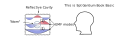
\includegraphics[scale=1.0]{defaultFigureTemplate}
  \caption{Operators extend the idea of functions. (a) An unary
    function $f$ can be applied to a number $x$ to produce
    another number $y$. (b) An unary operator $\op{F}$ can be applied to a vector
    $\vec{a}$ to yield another vector $\vec{b}$.}
  \label{fig:arrowsOperatorGeneral}
\end{figure}

\section{System}\label{sec:System}
A part of nature that can be clearly isolated and studied is called a \emph{physical system}. An electron, an atom, a molecule, a crystal, a pendulum, a comet, a star – these are examples of physical systems of various degrees of complexity.

Often a physical system is a body or several bodies interacting with each other or with some external bodies. Figure \ref{fig:systemExamples} provides several examples of \emph{mechanical systems}. Let’s examine them in more detail.
\begin{figure}[htbp]
	\centering
	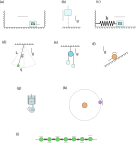
\includegraphics[scale=1.0]{systemExamples}
	\caption{Examples of mechanical systems. See text for explanation..}
	\label{fig:systemExamples}
\end{figure}
\renewcommand{\labelenumi}{(\alph{enumi})}
\begin{enumerate}
	\item \emph{Free falling body}: An elastic body falls down vertically under the
	force of gravity, bounces back, goes up and then down to repeat the
	bounce again and again. Also, a projectile launched at an angle.
	\item \emph{String pendulum}: A compact body is attached to a string
	of fixed length. It is allowed to swing back and forth without
	experiencing air friction.
	\item \emph{Atwood machine}: Two bodies with slightly unequal masses
	are connected with a non-stretchable string going over a
	frictionless pulley.
	\item \emph{Inclined plane}: A solid cylinder rolling down an
	inclinded plane.
	\item \emph{Piston}: A system of three bodies (cylindrical
	crankshaft, rod, and piston) connected in a way that locks rotation
	of a cylinder and the vertical motion of the piston.
	\item \emph{Spring oscillator}: A body, attached to a spring, is
	allowed to slide left and right across a frictionless surface.
	\item \emph{Linear chain of oscillators}: A set of pairwise
	interconnected identical bodies; the allowed motion happens along
	the horizontal axis.
	\item \emph{Sun and planet}: A planet circling around the sun.
	
\end{enumerate}
We will study oscillator and circular motion in great detail.

\subsection{Configuration}
In mechanics, \emph{configuration} means a formal way to describe the
arrangement of a system at a given time.

The behavior of a system in time can be described by specifying its
\emph{configuration} as the function of time. In relatively simple
systems, configuration may consist of a set of coordinates that uniquely
determine the arrangement of bodies in the system. For example, the
configuration of a pendulum can be given by a single coordinate --- the
length of the arc $q$. Of course, as the pendulum swings, both
Cartesian coordinates $x$ and $y$ are changing, but not independently,
due to the relation
\begin{equation*}
	x^2 + y^2 = L^2\, .
\end{equation*}
Given $x$, we can find $y > 0$ as $y = +\sqrt{L^2 - x^2}$, thus
reducing the number of required coordinates.

Consider another example, shown in the Figure
(\ref{fig:coupledSystem})(a): a system of
two bodies, connected with each other using ideal springs with
stiffness $k$, and each body is connected to a rigid wall.
\begin{figure}[htbp]
	\centering
	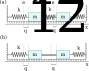
\includegraphics[scale=1.0]{coupledSystem}
	\caption{(a); (b).}
	\label{fig:coupledSystem}
\end{figure}

When the system is in equilibrium, the bodies occupy positions on the
horizotal axis denoted as $e_1$ and $e_2$. During motion, the position
of the first body changes by
\begin{equation*}
	q_1(t) = x_1(t) - e_1\, ,
\end{equation*}
and similarly for the second body: $q_2 = x_2 - e_2$. It is important
to realize, that although the two bodies are connected with a spring,
they can still move with different velocities, and have different
displacements $q_1 \ne q_2$. Indeed, we can set the system in motion
by moving each body independently and then releasing them. Contrast
this with the situation, shown in the Figure
(\ref{fig:coupledSystem})(b), where the bodies are connected with a
rigid rod, fusing two masses into essentially a single body. In this
case only a single displacement $q$ is required to specify the
configuration of the system.

\subsection{Qoordinates}
The coordinates specifying the configuration of a system do not
have to be Cartesian. In the example of a pendulum, the configuration
can be conveniently given by the length of the arc $q=L\theta$, see
Figure (\ref{fig:systemExamples})(b).

Consider another example, shown in the Figure
(\ref{fig:systemExamples})(h): Two bodies interact
gravitationally. In this problem, it turns out, the equations
describing the motion of the system are simpler if, instead of the
usual positions $x_1$ and $x_2$ we use the relative distance
\begin{equation*}
	q_1 = x_2 - x_1
\end{equation*}
and the position of the center of mass
\begin{equation*}
	q_2 = (m_1x_1 + m_2x_2)/(m_1 + m_2),
\end{equation*}
where $m_1$ and $m_2$ are the masses of the bodies.

We thus come to the idea of \emph{generalized coordinates} --
arbitrary coordinates completely specifying the configuration of a
system. Generalized coordinates can be based on positions, angles, or
some combinations of those.

\subsection{Degrees of Freedom}
\emph{Degree of freedom} is a separate independent motion of a
mechanical system. Each independent motion corresponds to the change
in time
of a separate generalized coordinate. The number of degrees of freedom
is the number of
generalized coordinates required to completely specify the
configuration of a mechanical system at different moments of time.

Take, for example, a pendulum, shown in the Figure
(\ref{fig:degreeOfFreedomPendulum}). In general Cartesian coordinates,
all three coordinates $x$, $y$, and $z$ will be changing in
time. However, only a single generalized coordinate $q(t)$ --- the
length of the arc -- is required to fully describe the configuration,
and thus the motion, of this mechanical system. The number of degrees
of freedom, in this example, equals 1.

\begin{figure}[htbp]
	\centering
	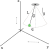
\includegraphics[scale=1.0]{degreeOfFreedomPendulum}
	\caption{A pendulum has one degree of freedom, despite the fact
		that all three Cartesian coordinates can be changing during its motion.}
	\label{fig:degreeOfFreedomPendulum}
\end{figure}




\section{Oscillator}\label{sec:Oscillator}
The model of an oscillator is extremely important. It appears in
various guises in almost all physical theories. Let's study it in details.

\begin{figure}[htbp]
	\centering
	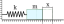
\includegraphics[scale=0.9]{Oscillator}
	\caption{A mechanical model of an oscillator: A body attached to an
		ideal spring.}
	\label{fig:Oscillator}
\end{figure}


Consider a body with the mass $m$ is attached to a spring with the stiffness
$k$. The body is allowed to move across a frictionless
surface.  The force required to strech a spring by the amount $x$
is given by the Hooke's law
\[
F=kx.
\]
This is the force applied \emph{to the spring}. The force created
\emph{by the spring, and applied to the attached body}, is of equal
magnitude but points in the opposite direction.

When the body is displaced from its equilibrium position,
by stretching or compressing the spring, and then released, it will
undergo periodic motion. During this motion, the position, velocity,
kinetic energy of the mody, and the potential energy of the spring
will be constantly changing.

To remind, the kinetic energy of a body is

\[
E_{k}=\frac{mv^{2}}{2}, \textrm{ or } K = \frac{p^2}{2m}\,.
\]
The potential energy of a spring, stretched or compressed by the
amount $x$ is given by

\[
E_{p}=\frac{kx^{2}}{2}, \textrm{ or } \Pi = \frac{kq^2}{2}\,.
\]


\section{State}\label{sec:State}
\emph{State} of a system is the \emph{minimal} collection of observables which is, in
certain sense, \emph{complete} and \emph{self-sufficient}. State is 
"all there is to know" about a system. If the state of a system is known at one
moment of time $t_0$, then we should be able to determine the state
at any later moment of time $t$. In classical mechanics the pair of
observables $(x, p)$ defines the state of a mechanical system.

\emph{State} is the minimal set of quantities describing mechanical
system and sufficient to predict
their future values from their initial values. State is an important
concept not only mechanics, but in other areas of physics.
Let's elaborate, using the oscillator as an example.

Suppose that at the moment of time $t_{0}$the position of the oscillator
is $x_{0}$ and its velocity is $v_{0}$. To find their values at
some later time $t>t_{0}$, we can go iteratevly in small steps, calculating
how much the position and the velocity change after each successive
tiny interval of time $\delta t$. The first iteration results in
the updated value of position
\begin{equation}
	x_{1}=x_{0}+v_{0}\delta t.
\end{equation}

The second, and every other, iteration looks very similar:
\begin{equation}
	x_{2}=x_{1}+v\delta t\,.
\end{equation}

Now it is important to realize that we can no longer use the same initial
velocity $v_{0}$in the second iteration, because the velocity itself
changes. Thus, we must update the value of the velocity as well. This
is done by using acceleration:
\begin{equation}
	v_{1}=v_{0}+a_{0}\delta t.
\end{equation}

Once this is done, we can find the second iteration of the position:
$x_{2}=x_{1}+v_{1}\delta t$. To keep this scheme going, we must be
able to update the value of the acceleration, because it is also changing.
It appears then, we need some quantity that allows to find the next
step:
\begin{equation}
	a_{1}=a_{0}+b_{0}\delta t,
\end{equation}
but, fortunately, \emph{this is not required!} At this point we can use the laws of motion.
For example, the Newton's second law allows us to find the acceleration,
if we know the force acting on the object:
\begin{equation}
	a=\frac{F}{m}.
\end{equation}

All physical forces, it appears, depend on positions (distances) and,
sometimes, velocities of bodies. The force of the spring $F=-kx$, for example,
depends only on the coordinate $x$. The force of gravitational interaction $F=GMm/r^2$
and the Coulomb force between two charges $F=kQq/r^2$ both depend on the distance
$r$ between the bodies. The force acting on an electron moving through
a magnetic field $F=qvB$ depends on the electron's velocity (and the field's strength $B$). 
No known forces depend on acceleration. This fact leads to an important conclusion:
It is enough to know position and velocity of an object at time $t_{0}$,
in order to find their values at any later moment of time $t>t_{0}$.
Obviously, position and velocity at any previous moment of time can
be found in the similar way.

Thus, we do not need to advance the acceleration by calculating its
small change $\delta a=b\delta t$, we can simply calculate it from
the law of motion:
\begin{equation}
	a_{n}=\frac{F(x_{n},v_{n})}{m}\,.
\end{equation}

This formula says that the acceleration at the iteration step number
$n$ is found from the values of the position $x_{n}$ and the velocity
$v_{n}$ at the same step. Given the velocity, we can advance the
postion, and given the acceleration, we can advance the velocity.
Then we recalculate the new value for the acceleration and repeat,
until we reach the final time $t$.

The preceding discussion demonstrates that in Newtonian mechanics
\emph{the state of a mechanical system} is given by a pair of quantities
-- $(x,v)$. There are alternatives to the Newtonian mechanics, and,
correspondingly, there are alternatives to the mechanical state. The
first such alternative is Hamiltonian dynamics.

\subsection{State Evolution: Newtonian Approach}
We will now apply the ideas and formulas of Newtonian mechanics to an
oscillator. We will calculate the motion of the oscillator in time
using a simple method of \emph{state evolution}. Specifically, we will
setup two simple equations -- one for position and one for velocity.

The equation for position is trivial and amounts to the definition:
\[
\frac{\delta x}{\delta t} = v\,.
\]
The equation for velocity follows from the second law of Newtonian
dynamics:
\[
\frac{\delta v}{\delta t} = \frac{F}{m} = -\frac{kx}{m}\,.
\]
Here we used the expression for the spring force $F=-kx$ acting
\emph{on the body} from the side of the spring.

Suppose we know the \emph{initial state} of the oscillator
$(x_0, v_0)$ at time $t_0=0$. When the clock makes a single tick after
a tiny time interval $\delta t$ the body will move to a new position
\[
x_1 = x_0 + v_0\delta t
\]
and the velocity will change due to the action of the spring:
\[
v_1 = v_0 -\frac{kx_0}{m}\,.
\]
Thus, after a single tick of the clock the state of the oscillator
will evolve from $(x_0, v_0)$ to $(x_1, v_1)$. At this point we can
keep repeat the steps to calculate the state after any number of
ticks, up to the desired time $t=N\delta t$.

We can now formalize the recipe for evolution of the state and write a
mathematical function
\[
(x_{new}, v_{new}) = f\, (x_{old}, v_{old}) = (x_{old}+v_{old}\delta
t, v_{old} - kx_{old}/m)\,.
\]
\begin{figure}[htbp]
	\centering
	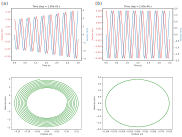
\includegraphics[scale=0.9]{newtonianStateEvolution}
	\caption{First row: Position (red curve, left axis) and velocity (blue
		curve, right axis) as functions of time. Second row: Velocity vs position.
		(a) Calculations with time step of 1 millisecond. (b) Calculations
		with time step of 1 microsecond.}
	\label{fig:newtonianStateEvolution}
\end{figure}

Using this simple approach, we can calculate the state $(x, v)$ of the
oscillator for any moment in the future or past. Figure
\ref{fig:newtonianStateEvolution} shows two example results. The first
result, in the column (a), demonstrates that we must be careful with
the step size $\delta t$ of the time. If it is not sufficiently small,
the inherent error of the method accumulates quickly, resulting in
wrong behavior, such as the gradual increase of velocity and
oscillation amplitude. The column (b) of Figure
\ref{fig:newtonianStateEvolution} demonstrates the expected behavior
of the oscillator -- periodic change of position with constant amplitude.

\section{Dynamics}\label{sec:Dynamics}
An action of an operator $F$ on arrows can be represented symbolically
as an equation.

\section{Hamiltonian}\label{sec:Hamiltonian}
An action of an operator $F$ on arrows can be represented symbolically
as an equation.

\section{Lagrangian}\label{sec:Lagrangian}
An action of an operator $F$ on arrows can be represented symbolically
as an equation.

\section{Field}\label{sec:Field}
An action of an operator $F$ on arrows can be represented symbolically
as an equation.

\section{Ideal Versus Real}\label{sec:IdealVsReal}
An action of an operator $F$ on arrows can be represented symbolically
as an equation.



\section*{Chapter Highlights}
{\setstretch{1.5}\chhc
  \it  
\begin{itemize}
\item Operators extends the idea of functions.
\item Numeric functions (e.g., $\sin\,x$) act on numbers and yield
  other numbers. Operators may act on vectors to yield other vectors
  or numbers.
\item Linear operators represent the simplest and yet powerful class
  of operators on vectors.
\item Linear operators can be represented graphically or symbolically.
\end{itemize}

}
